%%%%%%%%%%%%%%%%%%%%%%%%%%%%%%%%%%%%%%%%%%%%%%%%%%%%%%%%%%%%%%%
%%%  dts notes
%%%%%%%%%%%%%%%%%%%%%%%%%%%%%%%%%%%%%%%%%%%%%%%%%%%%%%%%%%%%%%%

\documentclass[onecolumn,fleqn]{revtex4}

% fonts
\usepackage{latexsym}
\usepackage{amsmath} 
\usepackage{amssymb} 
\usepackage{bm}
\usepackage{wasysym}

\usepackage{graphicx}


% extra by jarondl
\usepackage{array}
\usepackage{float}%unfloats
%\usepackage{multicol}
\usepackage[caption=false]{subfig} %subcaption is not compat with revtex
\usepackage[pdftitle={PTA},bookmarks]{hyperref}


%%%%%%%%%%%%%%%%%%%%%%%%%%%%%%%%%%%%%%%%%%%%%%%%%%%%%%%%%%%%%%%%

% NEW 
\newcommand{\abs}[1]{\left|#1\right|}
\newcommand{\varphiJ}{\bm{\varphi}}
\newcommand{\thetaJ}{\bm{\theta}}
%\renewcommand{\includegraphics}[2][0]{FIGURE}
\newcommand{\rmrk}[1]{\textcolor{red}{#1}}
\newcommand{\Eq}[1]{\textcolor{blue}{Eq.\!\!~(\ref{#1})}} 
\newcommand{\Fig}[1]{\textcolor{blue}{Fig.}\!\!~\ref{#1}}

% math symbols I
\newcommand{\sinc}{\mbox{sinc}}
\newcommand{\const}{\mbox{const}}
\newcommand{\trc}{\mbox{trace}}
\newcommand{\intt}{\int\!\!\!\!\int }
\newcommand{\ointt}{\int\!\!\!\!\int\!\!\!\!\!\circ\ }
\newcommand{\ar}{\mathsf r}
\newcommand{\im}{\mbox{Im}}
\newcommand{\re}{\mbox{Re}}

% math symbols II
\newcommand{\eexp}{\mbox{e}^}
\newcommand{\bra}{\left\langle}
\newcommand{\ket}{\right\rangle}

% Mass symbol
\newcommand{\mass}{\mathsf{m}} 
\newcommand{\rdisc}{\epsilon} 

% more math commands
\newcommand{\tbox}[1]{\mbox{\tiny #1}}
\newcommand{\bmsf}[1]{\bm{\mathsf{#1}}} 
\newcommand{\amatrix}[1]{\begin{matrix} #1 \end{matrix}} 
\newcommand{\pd}[2]{\frac{\partial #1}{\partial #2}}

% equations
\newcommand{\mylabel}[1]{\label{#1}} 
\newcommand{\beq}{\begin{eqnarray}}
\newcommand{\eeq}{\end{eqnarray}} 
\newcommand{\be}[1]{\begin{eqnarray}\ifthenelse{#1=-1}{\nonumber}{\ifthenelse{#1=0}{}{\mylabel{e#1}}}}
\newcommand{\ee}{\end{eqnarray}} 

% arrangement
\newcommand{\hide}[1]{}
\newcommand{\drawline}{\begin{picture}(500,1)\line(1,0){500}\end{picture}}
\newcommand{\bitem}{$\bullet$ \ \ \ }
\newcommand{\Cn}[1]{\begin{center} #1 \end{center}}
\newcommand{\mpg}[2][1.0\hsize]{\begin{minipage}[b]{#1}{#2}\end{minipage}}
\newcommand{\mpgt}[2][1.0\hsize]{\begin{minipage}[t]{#1}{#2}\end{minipage}}

%%%%%%%%%%%%%%%%%%%%%%%%%%%%%%%%%%%%%%%%%%%%%%%%%%%%%%%%%%%%%%%%%%%%%%%%%%%
% Sections
\newcommand{\sect}[1]
{
\addtocounter{section}{1} 
\setcounter{subsection}{0}
\ \\ 
\pdfbookmark[2]{\thesection. \ #1}{sect.\thesection}
{\Large\bf $=\!=\!=\!=\!=\!=\;$ [\thesection] \ #1}  
\nopagebreak
}

% subections
\newcommand{\subsect}[1]
{
\addtocounter{subsection}{1} 
\ \\ 
\pdfbookmark[2]{\ \ \ \ \thesection.\thesubsection. \ #1}{subsect.\thesection.\thesubsection}
{\bf $=\!=\!=\!=\!=\!=\;$ [\thesection.\thesubsection] \ #1}  
\nopagebreak
}
%%%%%%%%%%%%%%%%%%%%%%%%%%%%%%%%%%%%%%%%%%%%%%%%%%%%%%%%%%%%%%%%%%%%%%%%
%%%%%%%%%%%%%%%%%%%%%%%%%%%%%%%%%%%%%%%%%%%%%%%%%%%%%%%%%%%%%

\graphicspath{{figures/}}
\begin{document}

\title{PTA}

\author{YdL}

\maketitle

%%%%%%%%%%%%%%%%%%%%%%%%%%%%%%%%%%%%%%%%%%%%%%%%%%%%%%%%%%%%%%%%%%%%%%%%
%%%%%%%%%%%%%%%%%%%%%%%%%%%%%%%%%%%%%%%%%%%%%%%%%%%%%%%%%%%%%%%%%%%%%%%%


%%%%%%%%%%%%%%%%%%%%%%%%%%%%%%%%%%%%%%%%%%%%%%%%%%%%%%%%%%%
\sect{Model}

A periodic banded logbox model. The band profile is flat ($\Theta(b)$).
The off diagonal elements are log-box:
%
\begin{align}
w_{nm} &= w_0 \eexp{-\epsilon} \\
\epsilon &\in \textrm{uniform  } [0,2\sigma]
\end{align}
%
The diagonal elements are set so that each row's sum will be zero.
%
\begin{align}
w_{nn} = -\sum_{m\ne n} w_{nm}  
\end{align}
%
%%%%%%%%%%%%%%%%%%%%%%%%%%%%%%%%%%%%%%%%%%%%%%%%%%%%%
\sect{PN plots}

We have produced several plots of PN vs $\lambda$. For low-sparsity, there is an 
agreement with the two "windows" observation. (For very low sparsity there are even hints
of three windows). It seems that the effect of sparsity is to shorten the more extended window,
up to a point where very few modes are extended (remember that the special $\lambda=0$ is always fully extended).


\begin{figure}[H]
  \subfloat[Low sparsity]{
    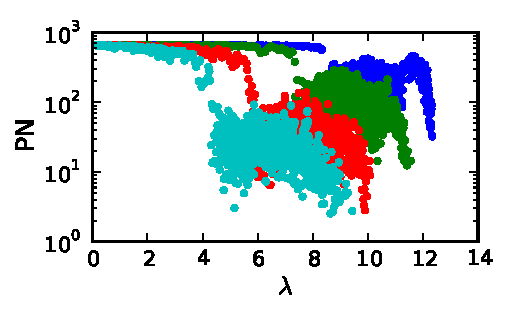
\includegraphics{pta_low_s_nopin}
    
  }
  \subfloat[Sparse]{
    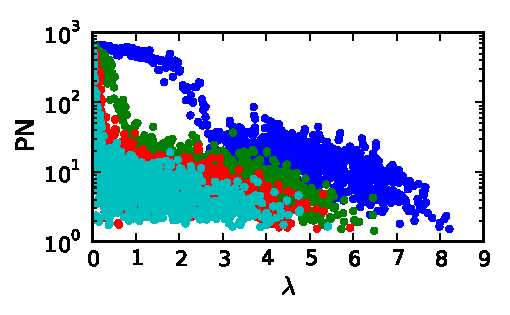
\includegraphics{pta_higher_s_nopin}
    
  }
  \\
  \subfloat[Very sparse]{
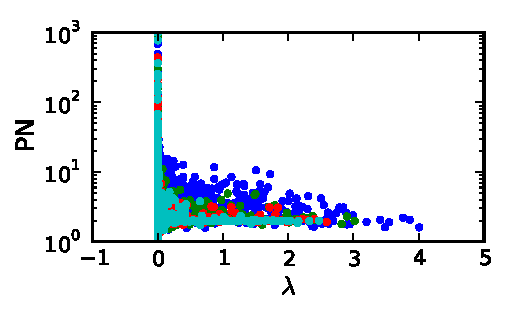
\includegraphics{pta_highest_s_nopin}
    
  }
\subfloat[Very sparse - logscale]{
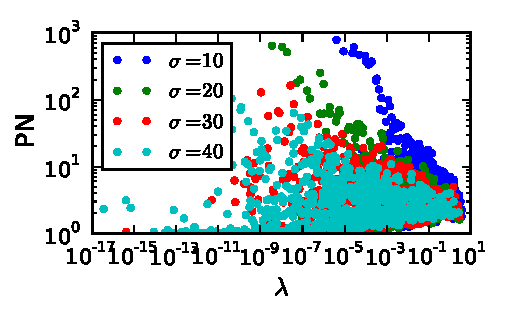
\includegraphics{pta_highest_s_log_nopin}
    
  }
  \caption{{\bf PN} as a function of $\lambda$ for sparse systems.
  For all the plots $N=1000$ and $b=5$}
\end{figure}



%%%%%%%%%%%%%%%%%%%%%%%%%%%%%%%%%%%%%%%%%%%%%%%%%%%%%%%%%%%%%%%%%%%%
\sect{The effects of pinning}

By pinning we mean adding some elements to the diagonal,
that represent a spring attaching a ball to a fixed origin.


We used a uniform distribution on the range $[-0.3,0]$,
in order to discern the effect.


It seems that the only difference is some localization in
the low-eigenvalues. The lowest modes are replaced with less 
extended modes with higher eigenvalues. Note that the $\lambda=0$ mode no longer
exist. To highlight the low eigenvalues,
we have used log-scale for the $\lambda$ axis.

\begin{figure}[H]
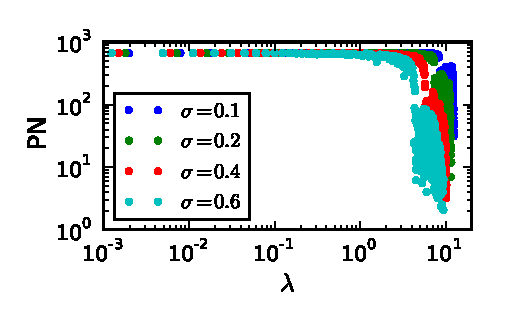
\includegraphics{pta_low_s_log_nopin}
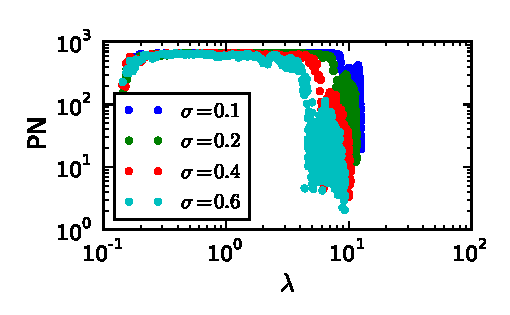
\includegraphics{pta_low_s_log_pin}
\caption{On the left, without pinning, and on the right with pinning}
\end{figure}


 
%%%%%%%%%%%%%%%%%%%%%%%%%%%%%%%%%%%%%%%%%%%%%%%%%%%%%%%%%%%%%%%%%%%
\sect{Thouless conductance}

Extended modes are more sensitive to boundary conditions. To measure
the effect quantitivly, we've used Thouless' method of adding
a phase to the boundary condition, and measuring the change in the eigenvalues.

We define $\lambda_0$ as the eigenvalue with regular periodic boundary conditions,
and $\lambda_\phi$ as the eigenvalue after applying a phase of $\phi$ to the boundary conditions.
Then $g$ is defined as
%
\begin{align}
  g = \frac{|\lambda_\phi - \lambda_0 |}{\phi^2}\ \times \ \frac{1}{\Delta}
\end{align}
%
Where $\Delta\ =\ \lambda_{n+1}-\lambda_n$ is the level spacing. 
In practice, we have averaged over five 
neighboring spacings to avoid artifacts.


The resulting $g(\lambda)$ is strikingly similar to the $PN(\lambda)$ results,
but the change is much stronger (note the logarithmic $y$-scale).  


\begin{figure}[H]
  \subfloat[Low sparsity]{
    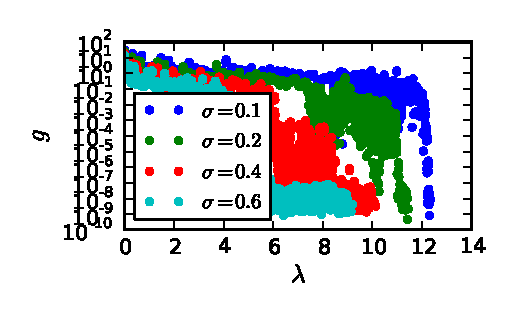
\includegraphics{pta_thouless_low_s}
    
  }
  \subfloat[Sparse]{
    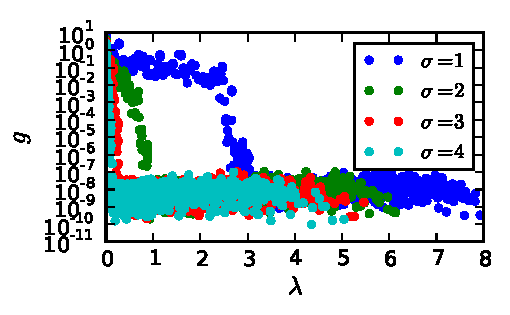
\includegraphics{pta_thouless_higher_s}
    
  }
  \\
  \subfloat[Very sparse]{
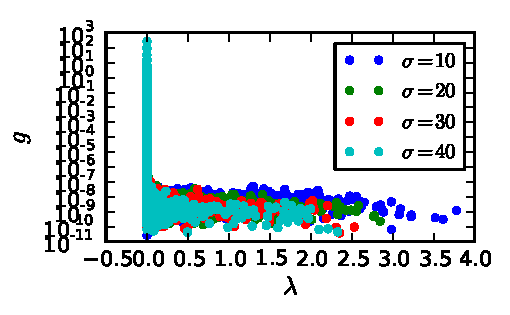
\includegraphics{pta_thouless_highest_s}
    
  }
\subfloat[Very sparse - logscale]{
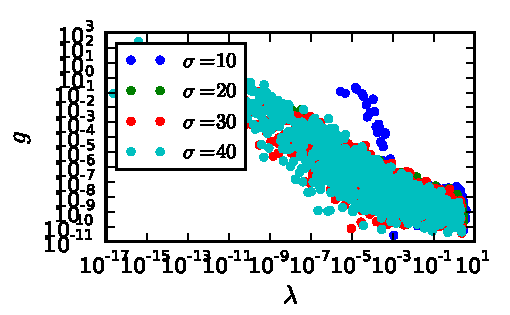
\includegraphics{pta_thouless_highest_s_log}
    
  }
  \caption{$g$ as a function of $\lambda$ for sparse systems.
  For all the plots $N=1000$ and $b=5$}
\end{figure}

%%%%%%%%%%%%%%%%%%%%%%%%%%%%%%%%%%%%%%%%%%%%%%%%%%%%%%%%%%%%%%%%%%%%%%%%%
\sect{Diagonal Disorder}


In the RP we have claimed that the conservation of the matrix
causes the very wide modes on the lower edge of the spectrum.
To see this point, we ran numerics with $N=1000$ $b=5$ and $\sigma=0.1$.

 Also notice the arc-like feature on the right,
it was there previously, but it is more pronounced for $\sigma=0.1$.  
The plateau is for $PN=\frac{2}{3}N$, as is expected for a cosine wave. 


Conservation means that the sum of each row is zero, so that the diagonal is minus the
sum of all other terms. The first way to break conservation is by adding
random elements to this diagonal.
\begin{align}
\gamma_n = -\sum_m w_{nm} + w_0\eexp{-\varepsilon}
\end{align}
 In the plot legends we mark this by the removal of $C$.
 
 
Another way is by neglecting to do the sum altogether,
keeping only:
\begin{align}
\gamma_n = + w_0\eexp{-\varepsilon}
\end{align}
In the plot legends we mark this by adding $D$.



In \autoref{fig:pta_sym1} we see the resulting $PN$ and $g$. We see
that the lowest eigenmodes behave differently. To examine this effect,
we have shifted the $x$ axis by the minimal $\lambda$, and applied log-scale.
For the conserving matrix, the $PN$ is constant in the low eigenvalues. The
uncoserving matrix has a small decline, and the one without special diagonal 
has a larger decline. 




\begin{figure}[H]
  \subfloat[g]{
    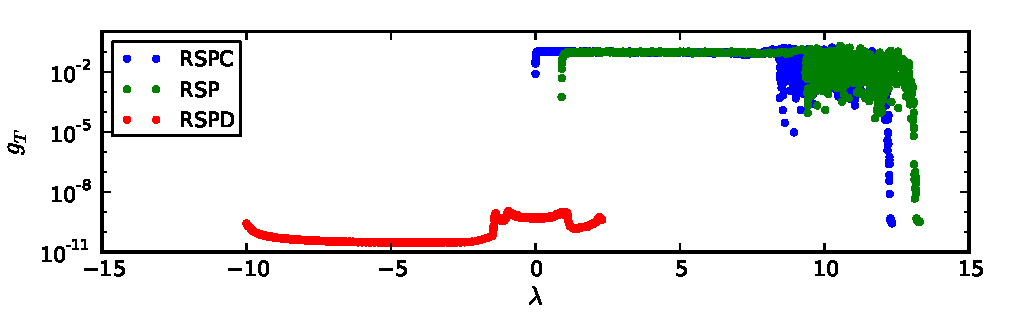
\includegraphics{pta_sym_neg_g}  
    
  }\\
  \subfloat[PN]{
    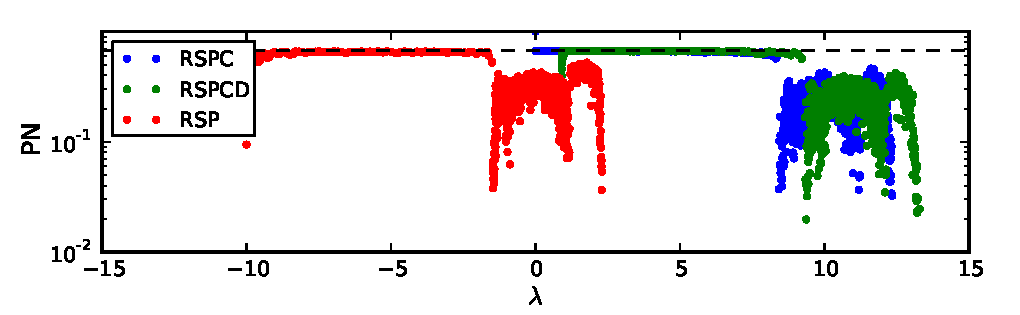
\includegraphics{pta_sym_neg_PN}
    
  }\\
  \subfloat[PN around zero]{
    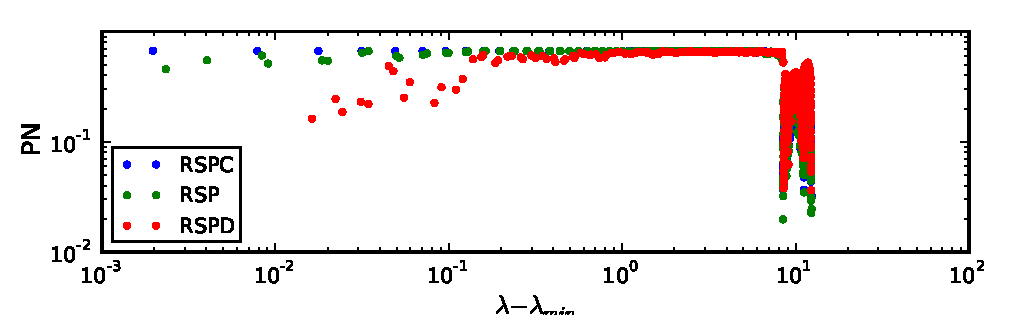
\includegraphics{pta_sym_neg_PN_zero}
    
  }
  \caption{$g$ and PN as a function of $\lambda$ for sparse systems.
  For all the plots $N=1000$, $b=5$ and $\sigma=0.1$. 
  The label codes are R-Real S-Symmetric P-[Positive Elements] C-Conservative D-[no-special diagonal] .
  The dashed line is on $y=2/3$, the expected PN for a cosine wave.}
  \label{fig:pta_sym1}
\end{figure}

%%%%%%%%%%%%%%%%%%%%%%%%%%%%%%%%%%%%%%%%%%%%%%%%%%%%%%%%%%%%%
\sect{non positive elements}

Here we check the effects of positivity on the $PN$ structure. We multiply
the matrix elements by a random sign $[\pm 1]$, keeping it symmetric.
The change from before is striking, as the plateau vanishes completely.

We examine the conservation aspects here as well, with the same
too measures of diagonal disorder. We see that when we do not treat the diagonal
specially, there are no wide modes at all. For the conserving and disorder matrices,
there are some wide modes. In the conserving case they are around the center, with a $\lambda=0, PN=N$ mode.
For the non-conserving mode this behavior shifts to the right. To further
analyze this area, we have shifted the $x$-axis, and plotted only the points to the 
right of the peak, to allow log-scale. The other half is symmetric. 
\begin{figure}[H]
  \subfloat[g]{
    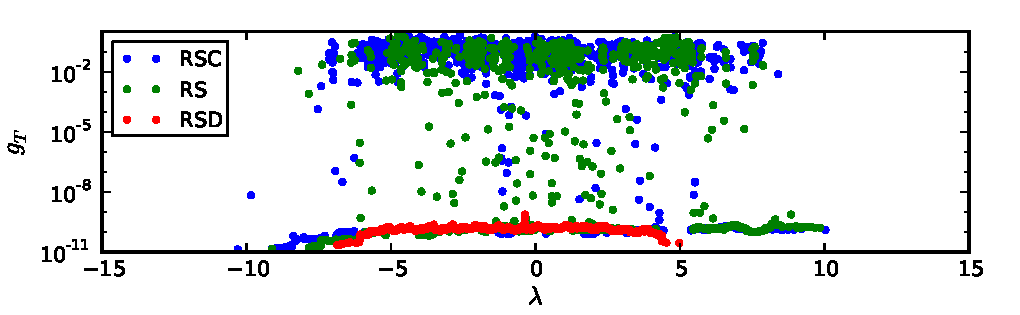
\includegraphics{pta_sym_neg_g2}  
    
  }\\
  \subfloat[PN]{
    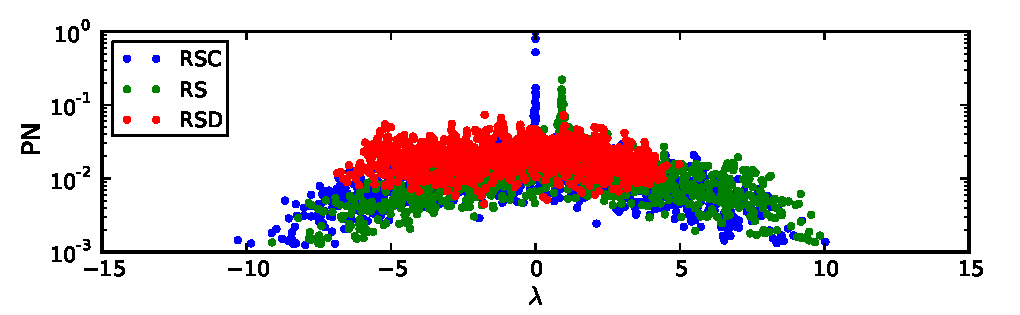
\includegraphics{pta_sym_neg_PN2}
    
  }\\
  \subfloat[PN around center]{
    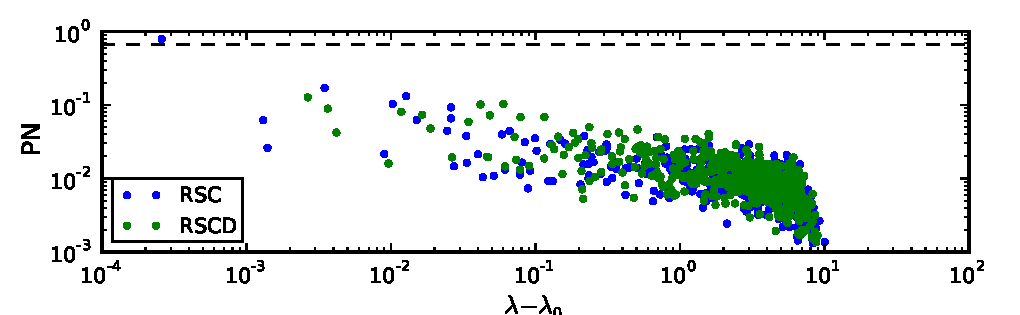
\includegraphics{pta_sym_neg_PN_center}
    
  }
  \caption{$g$ and PN as a function of $\lambda$ for sparse systems.
  For all the plots $N=1000$, $b=5$ and $\sigma=0.1$. 
  The label codes are R-Real S-Symmetric P-[Positive Elements] C-Conservative D-[no-special diagonal] . Note
  that the last plot has only half of the points}
  \label{fig:pta_sym2}
\end{figure}
\end{document}
